\documentclass[letter, 10pt]{article}
\usepackage{fullpage}
\usepackage[margin=0.5in]{geometry}
\usepackage{graphicx}
\usepackage{wrapfig}
\usepackage{caption}
\usepackage{subcaption}
\usepackage{listings}
\usepackage{hyperref}
\usepackage{amsmath}
\usepackage{float}

\pagenumbering{gobble}

\begin{document}
\noindent
\large \textbf{Rahul Ghosh} \hfill \textbf{Assignment\#2}\\
\normalsize Student ID: 5476965 \hfill CSci 5561\\

\section*{IMAGE REGISTRATION}
\subsection*{Methods}
Given an object/template, the aim of this project is to track the object/template in the given target frames as shown in Figure 1.

% \begin{figure}[!h]
%     \begin{center}
%         \includegraphics[width=0.45\textwidth]{HW2/RESULT/Frames.png}
%     \end{center}
%     \caption{Model Loss vs Global\_step}
% \end{figure}

We begin by computing the sift features of both the template and target images using the $vl\_feat$ library and pruning those images using the ration test and bidirectional consistency. The matched features between the Template and Target1 are shown in Figure 2.

% \begin{figure}[!h]
%     \begin{center}
%         \includegraphics[width=0.45\textwidth]{HW2/RESULT/MatchedFeatures.png}
%     \end{center}
%     \caption{Matched Features}
% \end{figure}

The images are now aligned using the features by calculating the transformation matrix A using RANSAC algorithm. The bounding box in Figure 3 shows the how the Template aligns with the Target Image. The target is then warped to the template image and the inital error image is shown in Figure 3.

% \begin{figure}[!h]
%     \begin{center}
%         \includegraphics[width=0.45\textwidth]{HW2/RESULT/AlignedWarpedImage.png}
%     \end{center}
%     \caption{Matched Features}
% \end{figure}

We refine the transformation matrix using the Inverse Compositional Image Alignment algorithm. The error plot over iterations is shown in Figure 4.

% \begin{figure}[!h]
%     \begin{center}
%         \includegraphics[width=0.45\textwidth]{HW2/RESULT/Error.png}
%     \end{center}
%     \caption{Matched Features}
% \end{figure}

For multiframe tracking we start with the original template and track it in Target1. We initialize the transformation matrix A using image alignment using features. For every target iteration we use a initial A and refine it using inverse compositional alignment. Now we update the template by warping the target image and also update the initial A using the refined A for tracking in the next frame. Figure 5 shows the updation of the tempate image and the tracked object is shown in Figure 6. 

\subsection*{RESULTS}

\begin{figure}[!h]
    \minipage{0.5\textwidth}
        \centering
        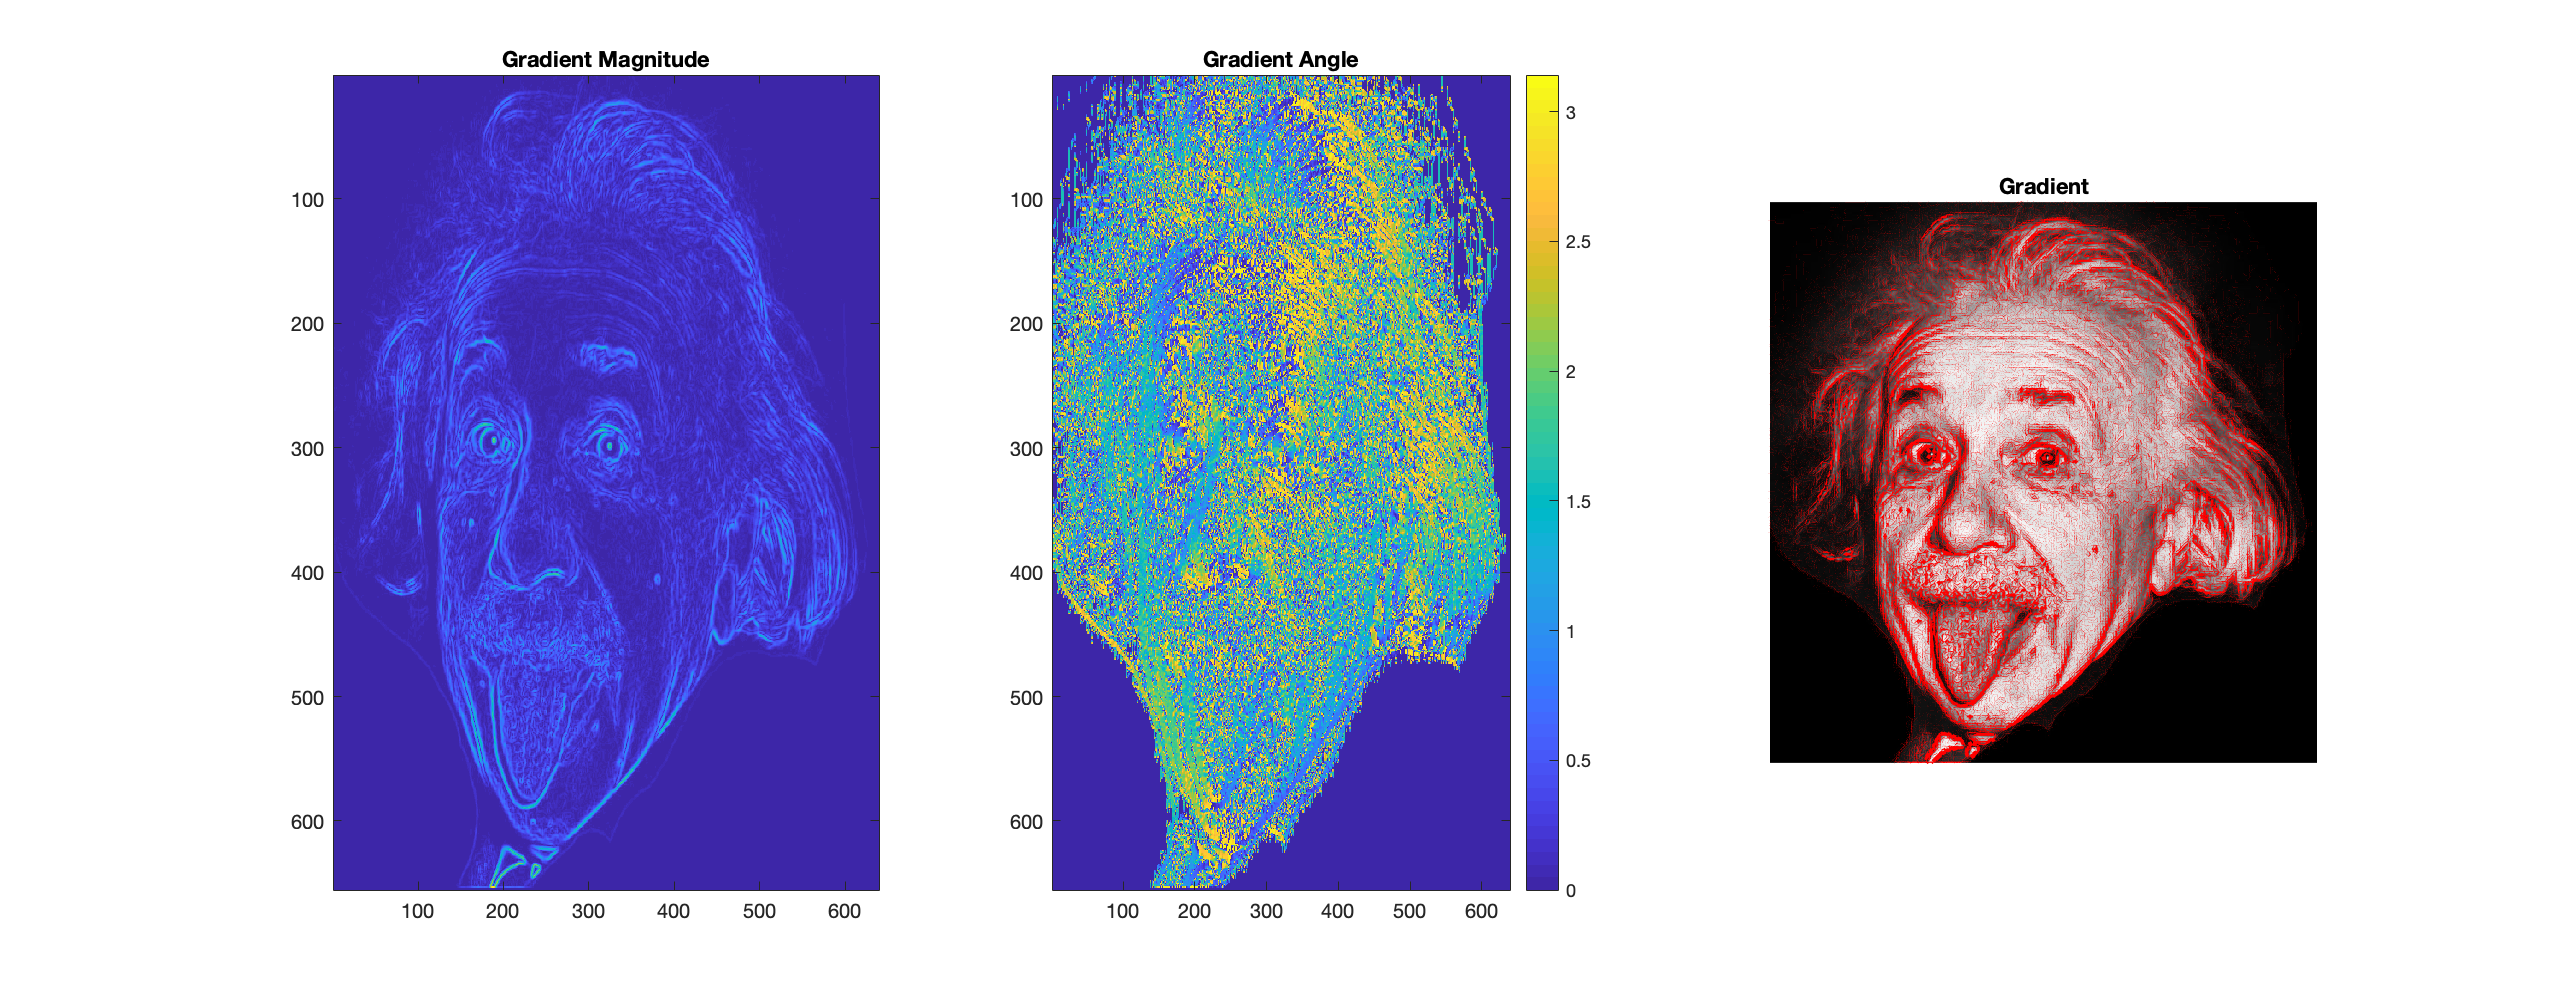
\includegraphics[width=\linewidth]{HW1/RESULT/GRADIENT.png}
        \subcaption{Gradients}
    \endminipage\hfill
    \minipage{0.25\textwidth}
        \centering
        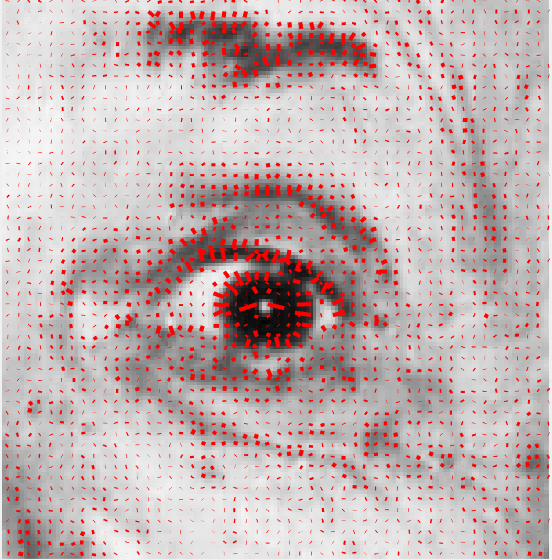
\includegraphics[width=0.7\linewidth]{HW1/RESULT/GRADIENT_EYE.png}
        \subcaption{Gradients\_EYE}
    \endminipage\hfill
    \minipage{0.25\textwidth}
        \centering
        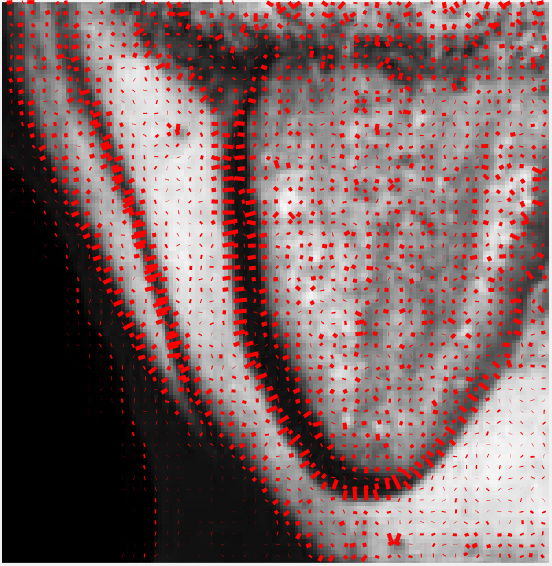
\includegraphics[width=0.7\linewidth]{HW1/RESULT/GRADIENT_TONGUE.png}
        \subcaption{Gradients\_TONGUE}
    \endminipage\hfill
    \caption{Gradients of Image}
\end{figure}

\end{document}